\documentclass[tikz, margin=2mm]{standalone}
\usepackage{tikz}
\usetikzlibrary{arrows.meta,backgrounds,matrix}

\begin{document}
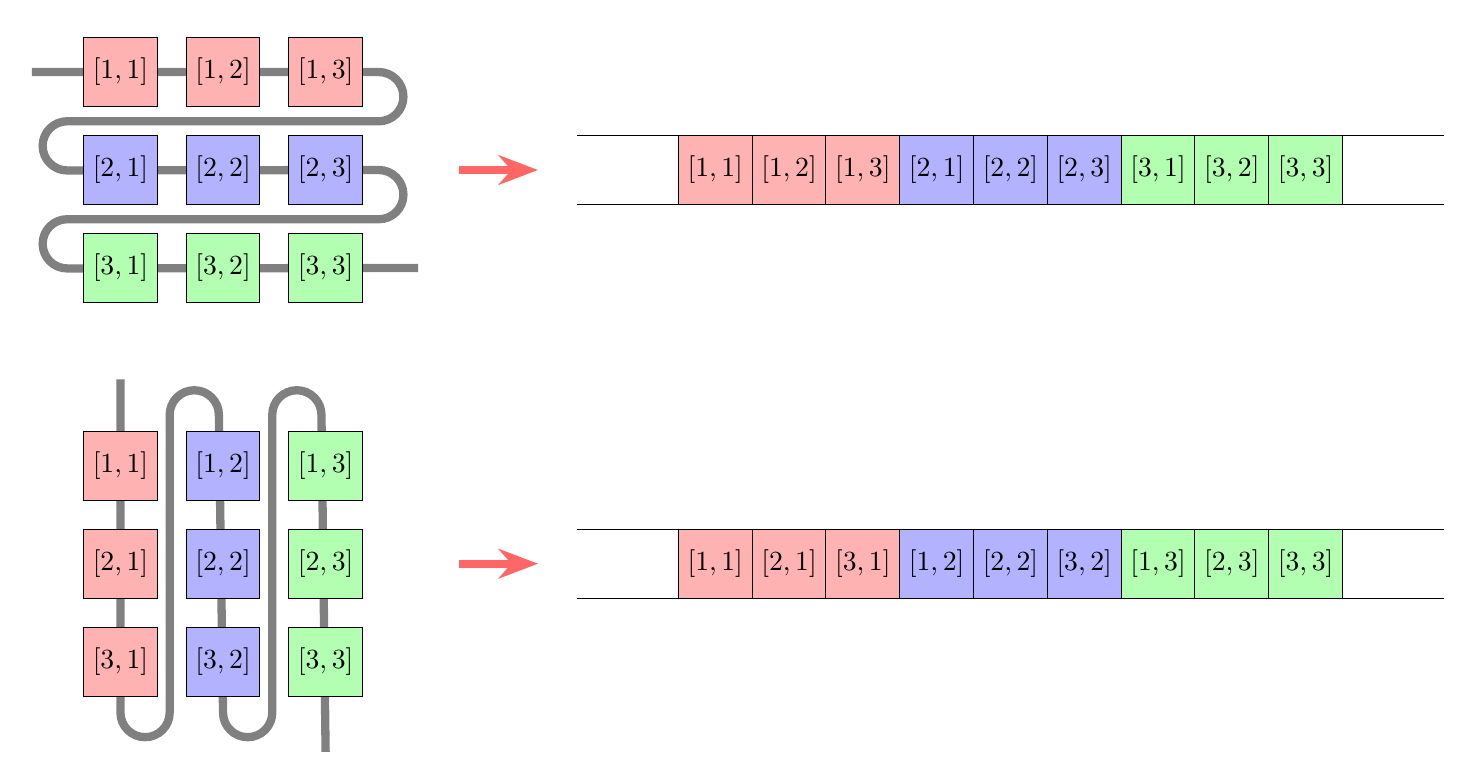
\begin{tikzpicture}[%
    arraynode/.style={
        draw,
        rectangle, 
        minimum size = 25,
        anchor = center,
        node contents={[\the\numexpr\pgfmatrixcurrentrow\relax,
                        \the\numexpr\pgfmatrixcurrentcolumn\relax]},
        alias=n\the\numexpr\pgfmatrixcurrentrow\relax\the\numexpr\pgfmatrixcurrentcolumn\relax
        },
    linearnode/.style={
        draw,
        rectangle, 
        minimum size = 25,
        anchor = center,
        },
    rowarray/.style={%
        matrix of math nodes,
        nodes = arraynode,
        column sep = 10,
        row sep = 10,
        nodes in empty cells,
        row 1/.style={nodes={fill=red!30}},
        row 2/.style={nodes={fill=blue!30}},
        row 3/.style={nodes={fill=green!30}},
        }, 
    columnarray/.style={%
        matrix of math nodes,
        nodes = arraynode,
        column sep = 10,
        row sep = 10,
        nodes in empty cells,
        column 1/.style={nodes={fill=red!30}},
        column 2/.style={nodes={fill=blue!30}},
        column 3/.style={nodes={fill=green!30}},
        }, 
    lineararray/.style={
        matrix of math nodes,
        nodes = linearnode,
        row sep = -\pgflinewidth,
        column sep = -\pgflinewidth,
        nodes in empty cells,
        column 1/.style={nodes={fill=red!30}},
        column 2/.style={nodes={fill=red!30}},
        column 3/.style={nodes={fill=red!30}},
        column 4/.style={nodes={fill=blue!30}},
        column 5/.style={nodes={fill=blue!30}},
        column 6/.style={nodes={fill=blue!30}},
        column 7/.style={nodes={fill=green!30}},
        column 8/.style={nodes={fill=green!30}},
        column 9/.style={nodes={fill=green!30}},
        },
]

\begin{scope}
    \matrix[rowarray] {
    &&\\
    &&\\
    &&\\
    };

    \begin{scope}[on background layer]
    \draw[line width=3pt, black!50] ([xshift=-6.5mm]n11.west)
            foreach \i [count=\ni from 1] in {1,...,2}{
            -- ([xshift=2mm]n\i3.east) arc(90:-90:3.125mm)
            -- ([shift={(-2mm,-6.25mm)}]n\i1.west) arc(90:270:3.125mm)}
            -- ([xshift=7mm]n33.east);
    \end{scope}
\end{scope}

\begin{scope}[yshift=-5cm]
    \matrix[columnarray] {
    &&\\
    &&\\
    &&\\
    };

    \begin{scope}[on background layer]
    \draw[line width=3pt, black!50] ([yshift=6.5mm]n11.north) 
    foreach \i [count=\ni from 1] in {1,...,2}{
    -- ([yshift=-2mm]n3\i.south) arc(180:360:3.125mm)
    -- ([shift={(6.25mm,2mm)}]n1\i.north) arc(180:0:3.125mm)}
    -- ([yshift=-7mm]n33.south);
    \end{scope}
\end{scope}

\begin{scope}[xshift=3cm]
    \draw [-{Stealth[length=5mm]}, line width=3pt, red!60] (0,0) -- (1,0);
\end{scope}

\begin{scope}[xshift=10cm]
    \draw[black] (-5.5,+12.5pt) -- (+5.5,+12.5pt);
    \draw[black] (-5.5,-12.5pt) -- (+5.5,-12.5pt);

    \matrix [lineararray] {
        {[1,1]} & {[1,2]} & {[1,3]} & {[2,1]} & {[2,2]} & {[2,3]} & {[3,1]} & {[3,2]} & {[3,3]} \\
    };
\end{scope}

\begin{scope}[xshift=3cm, yshift=-5cm]
    \draw [-{Stealth[length=5mm]}, line width=3pt, red!60] (0,0) -- (1,0);
\end{scope}

\begin{scope}[xshift=10cm, yshift=-5cm]
    \draw[black] (-5.5,+12.5pt) -- (+5.5,+12.5pt);
    \draw[black] (-5.5,-12.5pt) -- (+5.5,-12.5pt);

    \matrix [lineararray] {
        {[1,1]} & {[2,1]} & {[3,1]} & {[1,2]} & {[2,2]} & {[3,2]} & {[1,3]} & {[2,3]} & {[3,3]} \\
        };
\end{scope}

\end{tikzpicture}%
\end{document}
